\documentclass[conference]{IEEEtran}
\IEEEoverridecommandlockouts                              
%\overrideIEEEmargins
\usepackage[utf8]{inputenc}
\usepackage[T1]{fontenc}
\usepackage{hyperref}
\usepackage{xcolor}
\usepackage{graphicx}
\usepackage{amsmath}
\graphicspath{{./images/}}

\begin{document}
\title{Exploitation - Exploration in simple n-arm
bandit reinforcement learning $|$ Epsilon-Greedy Algorithm}
% author names and affiliations
\author{\IEEEauthorblockN{Mukesh Vaishnav}
\IEEEauthorblockA{202051196}
\and
\IEEEauthorblockN{Kaushik Rathva}
\IEEEauthorblockA{202051156}
\and
\IEEEauthorblockN{Patel Jaykumar}
\IEEEauthorblockA{202051136}
\and
\IEEEauthorblockN{Sontakke Ajinkya}
\IEEEauthorblockA{202051179}
}
% make the title area
\maketitle
\setlength{\parindent}{20pt}
\noindent Github link: \href{https://github.com/JARVIS-codebase/LAB-5}{LAB-9} \\ \\ 
\indent \begin{abstract}
In particular, the n-arm bandit problem is used in this lab to better grasp the terms exploitation and exploration in the context of reinforcement learning. The epsilon-greedy algorithm, a well-known exploration-exploitation tactic in reinforcement learning, will be the subject of the study.
\end{abstract}
\IEEEpeerreviewmaketitle

\section{Introduction}
An example of a classic reinforcement learning issue is the "n-arm bandit problem," which involves a collection of n slot machines or "one-armed bandits" with various payoff probabilities. By playing the machines frequently and taking lessons from the results, the objective is to identify the machine with the largest expected payoff.\\
Choosing the machine with the largest estimated payoff based on the available information is known as exploiting. The goal of exploration, on the other hand, is to select machines with lower anticipated rewards in order to learn more about their actual reward possibilities. \\
A straightforward technique that balances exploitation and exploration is the epsilon-greedy algorithm. With a probability of 1-epsilon, the algorithm chooses the machine with the largest estimated payoff, and with an epsilon probability, it chooses a machine at random.
\section{Problem Statement-1} 
Consider a binary bandit with two rewards 1-success, 0-failure. The bandit returns 1 or 0 for the action that you select, i.e. 1 or 2. The rewards are stochastic (but stationary). Use an epsilon-greedy algorithm discussed in class and decide upon the action to take for maximizing the expected reward. There are two binary bandits named binaryBanditA.m and binaryBanditB.m are waiting for you.\\
\\
Using epsilon-greedy algorithm, we follow:
\begin{enumerate}
    \item Define the epsilon value, which determines the probability of taking a random action instead of the greedy action that maximizes the expected reward. \\
    For instance, epsilon = 0.2 means that there is a 20\% chance of taking a random action. \\
    \item Initialize the expected rewards for each action in each bandit to zero. This can be done using a 2x2 matrix. \\
    \item Repeat the following steps for a fixed number of iterations or until convergence:
    \begin{enumerate}
    \item With probability epsilon, select a random action. Otherwise, select the action with the highest expected reward (the greedy action).
    \item Observe the reward from the selected action and update the expected reward for that action using a simple average of the previous reward and the new reward.
    \end{enumerate} 
    \item After the iterations are completed, select the bandit with the highest expected reward.
\end{enumerate} 
The following findings were drawn from the use of reward functions binaryBanditA and binaryBanditB: \\
When the likelihood of a reward was low for banditA, the initial expected rewards were zero. However, the expected rewards increased along with the number of trials. \\
The projected rewards for banditB, on the other hand, were near 1 at the start because of the high reward probability (0.8 and 0.9). The averaging factor ensured that the expected benefits were constant as the number of steps rose.
$$Iterations:500\; Epsilon:0.2$$
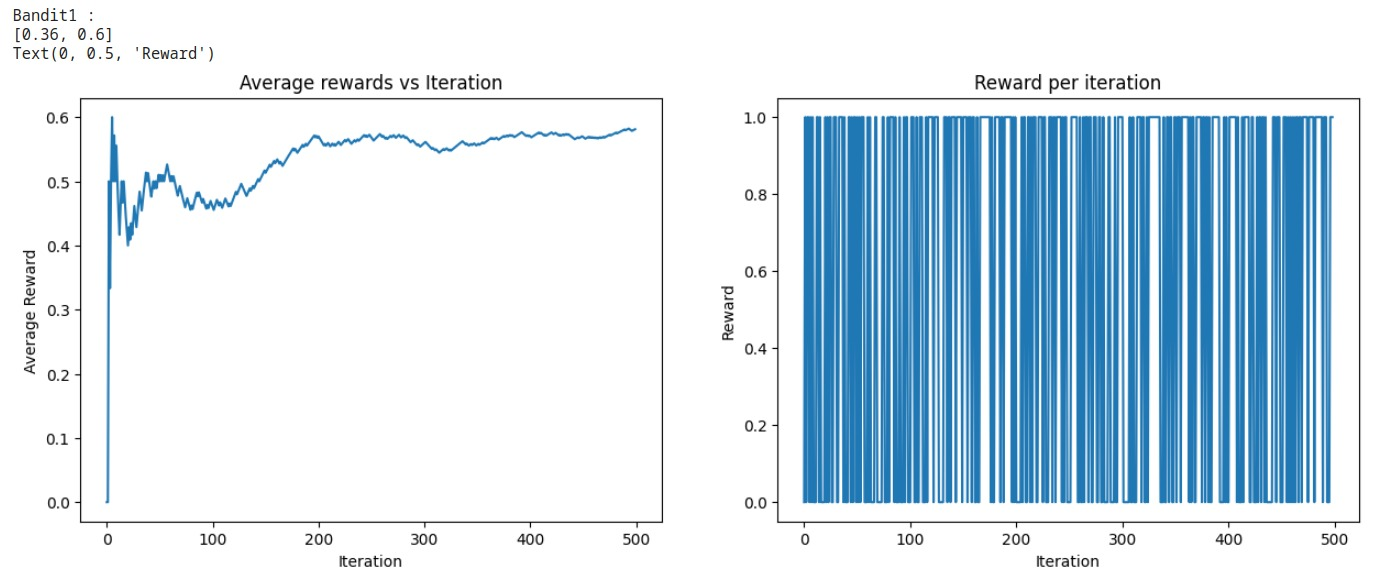
\includegraphics[scale=0.2]{images/9.1.jpg}
$$Fig. \; Rewards \; using \; banditA$$
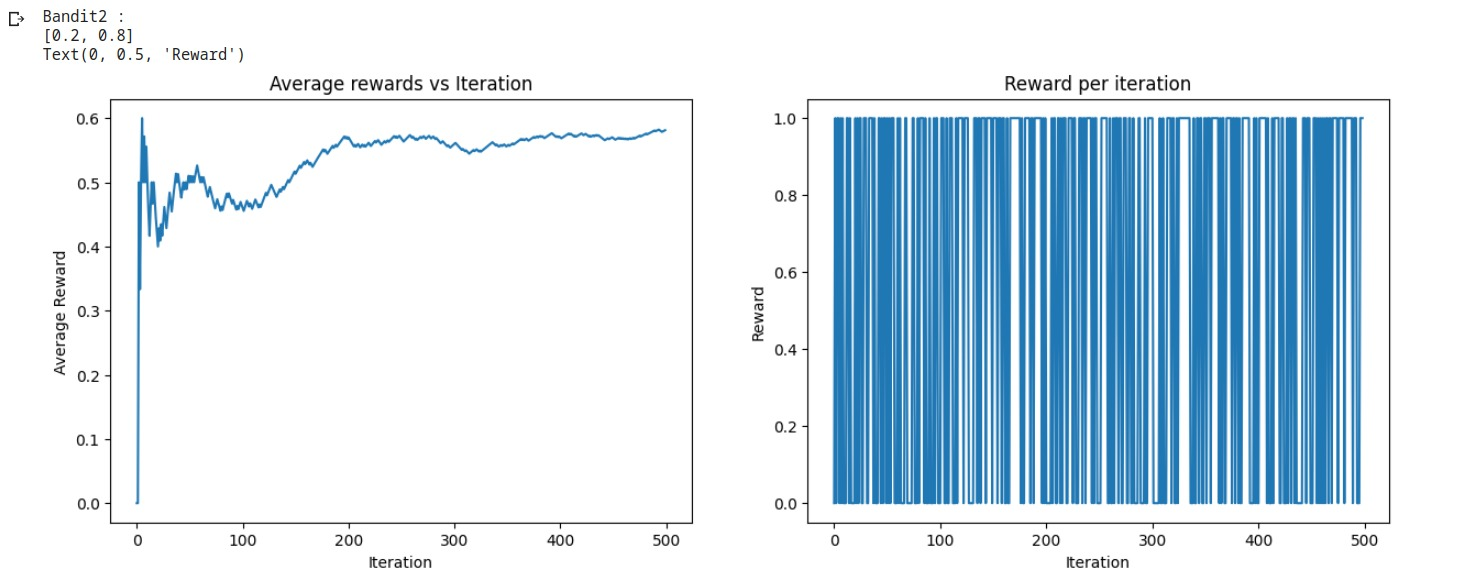
\includegraphics[scale=0.2]{images/9.2.jpg}
$$Fig. \; Rewards \; using \; banditB$$
$$Iterations:100\; Epsilon:0.2$$
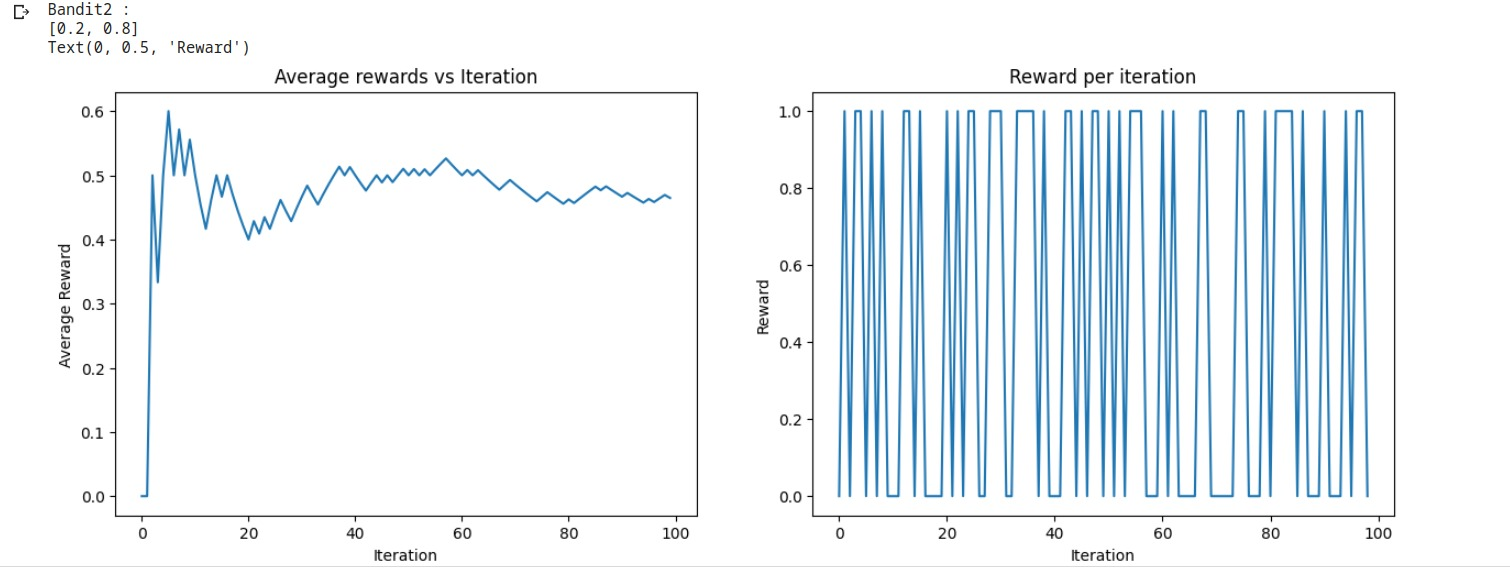
\includegraphics[scale=0.18]{images/9.3.jpg}
$$Fig. \; Rewards \; using \; banditA$$
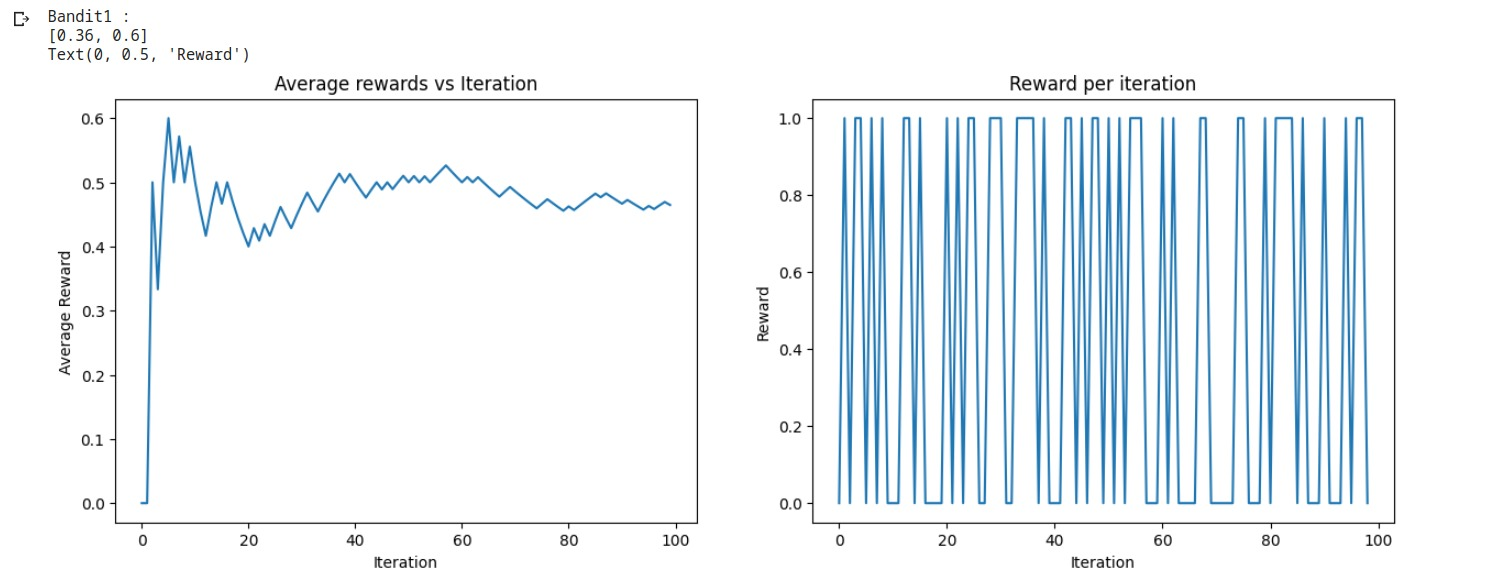
\includegraphics[scale=0.18]{images/9.4.jpg}
$$Fig. \; Rewards \; using \; banditB$$

\section{Problem Statement-2} 
Develop a 10-armed bandit in which all ten mean-rewards start out equal and then take independent random walks (by adding a normally distributed increment with mean zero and standard deviation 0.01 to all mean-rewards on each time step). 
\{function [value] = bandit\_nonstat(action)\}\\ 
\\
With a reward method that returns a reward for a specific arm index and an incrementReward method that updates the mean rewards of each arm by adding a normally distributed increment with mean zero and standard deviation 0.01, the Bandit class represents the 10-armed bandit. The reward is taken from a normal distribution, with a mean equal to the arm's current mean reward and a standard deviation of 1.\\
For a ten-arm bandit, the mean-rewards are initially set to a fixed array with a value of 1. The Epsilon Greedy Algorithm is used to conduct the exploration and exploitation. A random integer between 0 and 1 is created to determine whether to exploit or explore, and if it exceeds epsilon, exploitation is carried out using prior knowledge. A ten-value array with a mean of zero and a standard deviation of 0.1 that is normally distributed is created after each iteration. Following actions that provide incentives based on the updated mean-rewards array use the updated array, which is added to the mean array. In this case, the prizes are not stationary.\\ \\ \\ \\ \\ \\ \\ \\
$$Iterations:20000$$
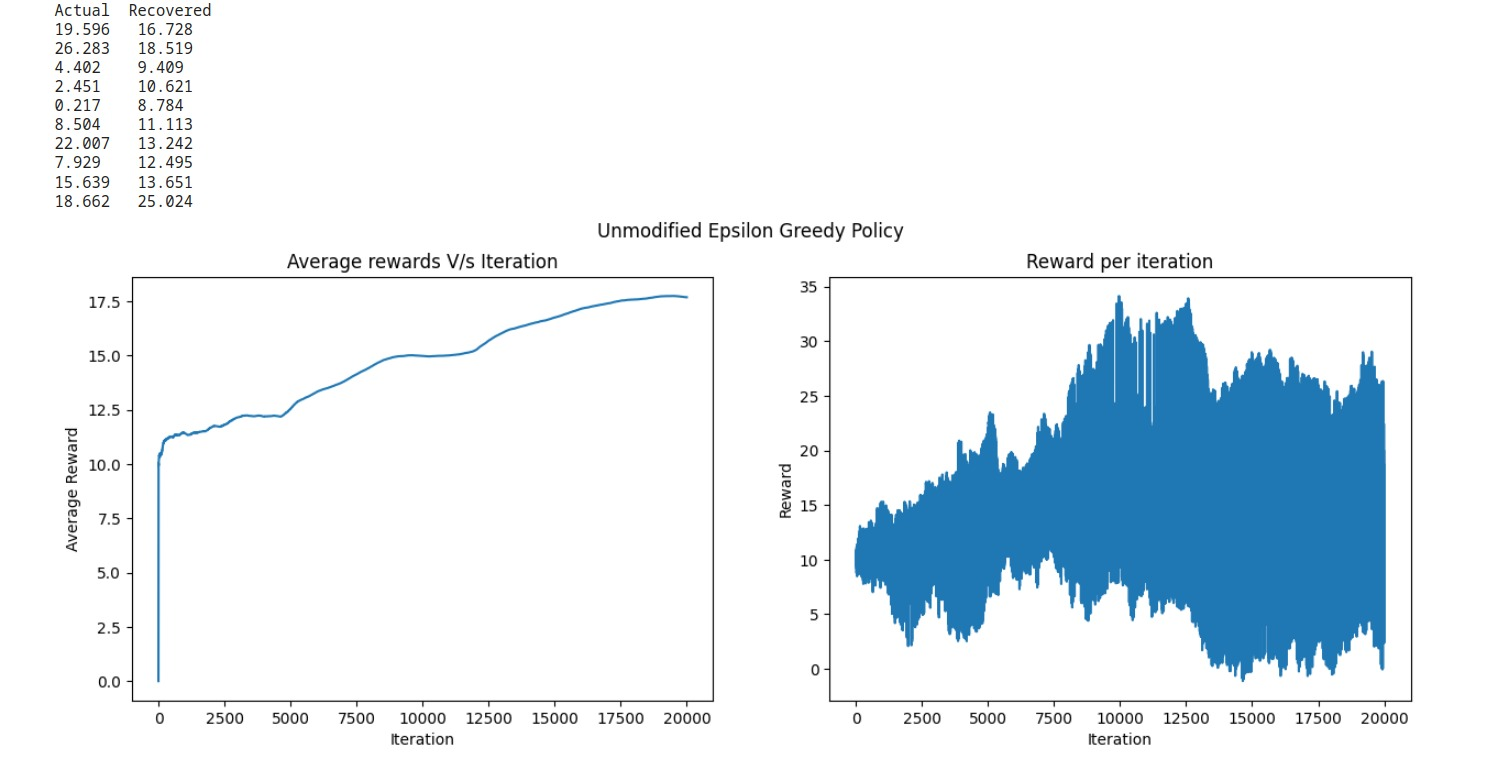
\includegraphics[scale=0.18]{images/9.5.jpg}
$$Fig. \; Ten \; Armed \; Bandit$$
As we can see, at first, all rewards are equal to 0, but as the number of iterations rises, each action's rewarding policy is altered, and the expected payouts rise at a quick, non-zero rate.\\
\section{Problem Statement-3} 
The 10-armed bandit that you developed (bandit\_nonstat) is difficult to crack with a standard epsilon-greedy algorithm since the rewards are non-stationary.  We did discuss how to track non-stationary rewards in class.  Write a modified epsilon-greedy agent and show whether it is able to latch onto correct actions or not.  (Try at least 10000 time steps before commenting on results)\\ 
\\
This problem, in contrast to Problem 2, updates the action reward estimation by giving the current earned reward more weight by using the alpha parameter as opposed to the average method in the latter.\\  \\
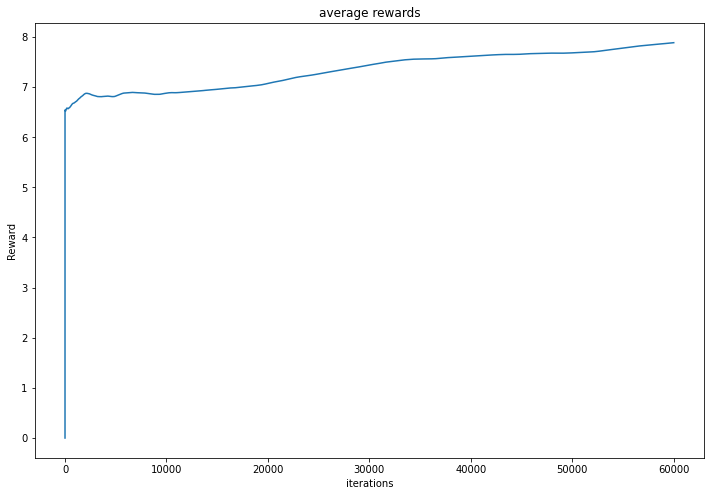
\includegraphics[scale=0.35]{images/9.6.png}
$Fig. \; Expected \; rewards \; we \; get \; when \; rewards \; are \; non-stationary\; (averaging\; method)$
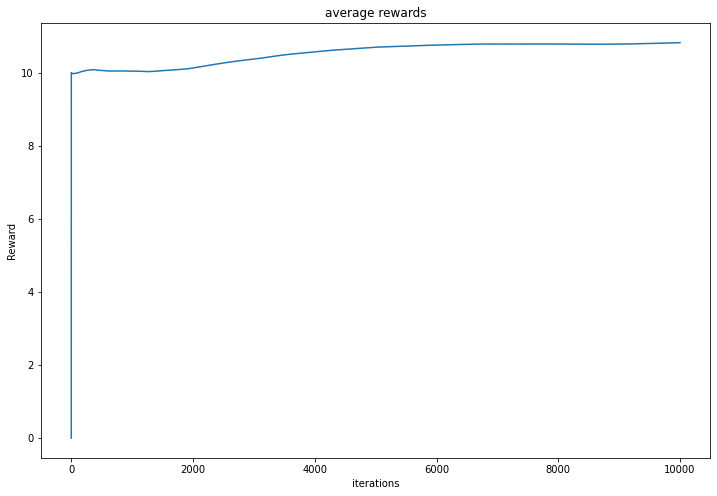
\includegraphics[scale=0.35]{images/9.7.png}
$Fig. \; Expected \; rewards \; we \; get \; when \; rewards \; are \; non-stationary \; (non-averaging \; method)$ \\ \\
In question 3, the predicted rewards were substantially higher than in question 2, and the graph's gradient was much steeper than in question 1. 
\section{CONCLUSION}
A straightforward but significant problem in reinforcement learning is the n-arm bandit problem. This issue can be resolved and the balance between exploitation and exploration balanced using the epsilon greedy algorithm. The n-arm bandit problem can be solved using the epsilon greedy method using the basic framework provided by this implementation.
\begin{thebibliography}{}
\bibitem{}
Richard S. Sutton and Andrew G. Barto (2014, 2015) \emph{Reinforcement Learning: An Introduction}, Bradford, The MIT Press, Cambridge, Massachusetts, London, England
\bibitem{}
Tanmay Ambadkar (2021) Artificial Intelligence Course. \href{https://github.com/TanmayAmbadkar/CS302-AI/tree/master/Lab9}{https://github.com/TanmayAmbadkar/CS302-AI/tree/master/Lab9}(2021).
\end{thebibliography}
\end{document}


